\chapter{Wizualizacja przy pomocy warstw ukrytych sieci VGG-19}
\label{chap:vgg}
\section{Model sieci VGG-19}
\label{vgg-model}

Do bardziej złożonych wizualizacji posłużę się siecią VGG, której architekturę zaprezentowano po raz pierwszy w 2015 roku w publikacji autorstwa Karen Simonyan i 
Andrew Zisserman\cite{vggpaper}. W publikacji zaprezentowano kilka wariantów tej sieci. Ja z uwagi na większą ilość warstw użyję wariantu VGG-19.

\begin{figure}[ht]
\centerline{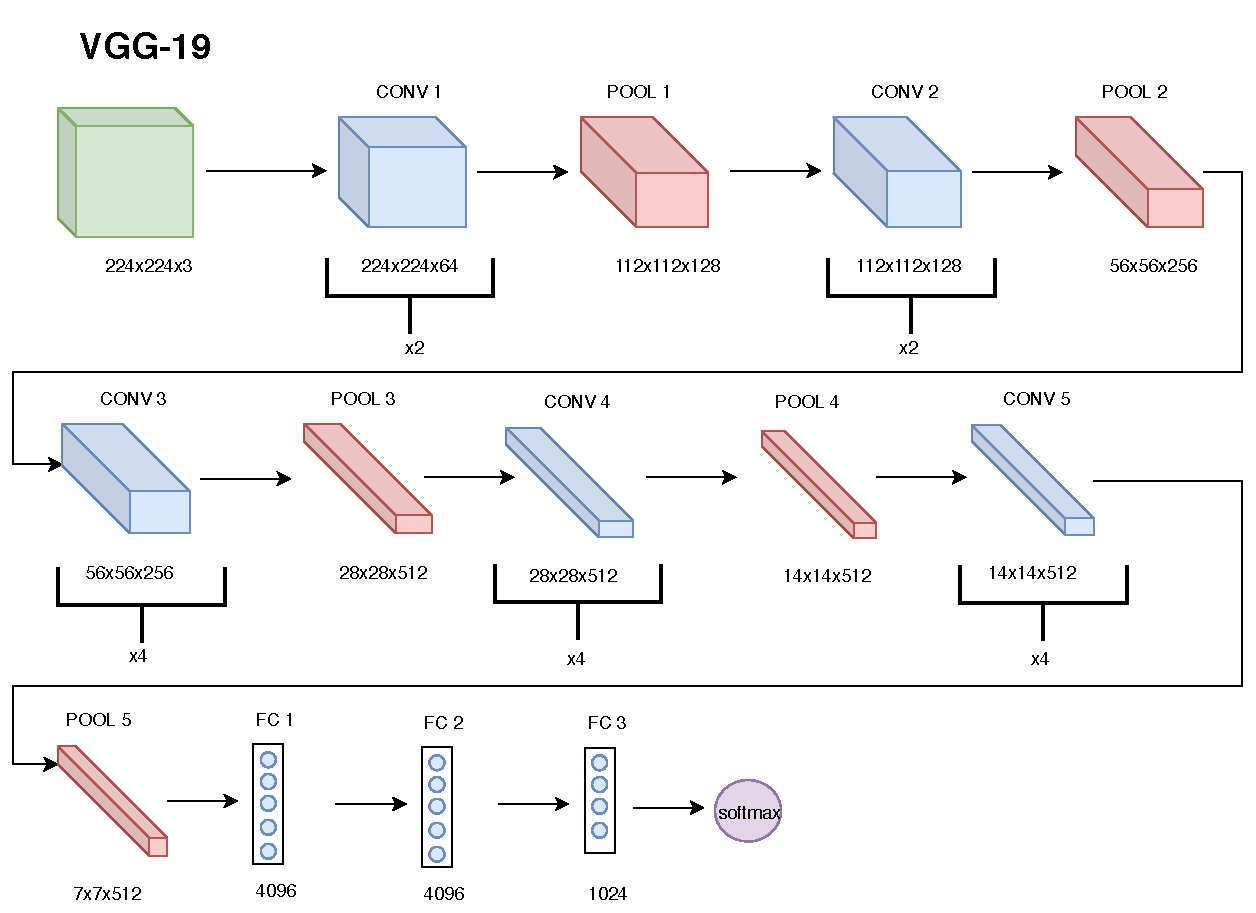
\includegraphics[scale=0.5]{resources/vgg/vgg.pdf}}
\caption{Schemat modelu sieci VGG-19.}
\label{fig:vgg19-schemat}
\end{figure}

Dopełnienie w przypadku warstw konwolucyjnych wynosi \(p=1\) przy skoku \(s=1\) co sprawia, że warstwy konwolucyjne mogą być ze sobą łączone w łańcuchy niezmieniające wymiarów tensora. W przypadku warstw \textit{poolingowych} \(p=1\) przy skoku \(s=2\) tym samym, dzielą one dwa pierwsze wymiary przez pół. Sumarycznie daje to 16 warstw możliwych do wykorzystania w wizualizacjach.

\subsection{Wizualizacja poprzez rekonstrukcję obrazu przy pomocy maksymalizacji aktywacji neuronu}
\label{vgg-mean-activation}

Z racji swoich rozmiarów, trening sieci VGG zajmuje dni, nawet przy pomocy GPU. Użyję więc wcześniej wytrenowanej sieci dostępnej bezpośrednio w Kerasie.

\label{lst:vggkeras}
\begin{lstlisting}[language=Python, caption={Wczytywanie wag VGG-19 w Keras.}, captionpos=b]
from keras.applications import VGG19
model = VGG19(include_top=False, weights='imagenet')
\end{lstlisting}

Zastosowane opcje to przede wszystkim zestaw danych na, których była trenowana sieć, w tym wypadku zbiór ImageNet\cite{imagenet}, oraz wyłączenie z ładowanego modelu warstw gęstch. Ta ostatnia opcja pozwoli na rekonstukcję obrazu o dowolnej liczbie pikseli (zamiast standardowego dla architektury VGG 224\(\times\)224 pikseli).

Mając załadowany model wraz z wytrenowanymi wagami, wybieram poszczególne filtry z kolejnych warstw konwolucyjnych. Następnie, generuję losowy (wartość pikseli losowana jest z rozkładu jednorodnego) obrazek o niskiej rozdzielczości, początkowo szary obraz zaburzam nieznacznie różnymi kolorami i wyliczam aktywacje wybranej wcześniej warstwy.
Przykładowy obraz wejściowy przedstawia rysunek \ref{fig:obrazwe}

\begin{figure}[ht]
\centerline{
\includegraphics[scale=1]{resources/cnn/obrazwe.png}}
\caption{Obraz wejściowy dla skryptu maksymalizującego medianę warstwy.}
\label{fig:obrazwe}
\end{figure}

Medianę z tych aktywacji traktuję jako wartość mojej funkcji kosztu i modyfikuję wylosowany uprzednio obrazek w celu jej maksymalizacji.

Maksymalizacja aktywacji jest możliwa poprzez wywołanie metody o nazwie \textit{gradients} z biblioteki Keras. Wykorzystując ją można przy pomocy tensora wejściowego, w tym wypadku zdjęcia, oraz funkcji kosztu (zdefiniowanej powyżej) uzyskać gradient funkcji kosztu dla danych z tensora.Następnie, moim celem będzie wykonać operację odwrotną niż w podczas treningu sieci -- maksymalizację funkcji kosztu. Uzyskany gradient wykorzystywany jest do przekształcania obrazu.

Modyfikacja obrazu polega na dodaniu odpowiednio znormalizowanego gradientu do wartości poszczególnych pikseli. Cały proces treningu składa się z kilkukrotnego skalowania obrazu do wyższych ,,rozdzielczości'' i ponawiania procesu optymalizacji. 

Skalowanie jest konieczne, ponieważ struktury generowane tą metodą charakteryzują się wysoką częstotliwością (są małe i powtarzalne). Uprzednie wygenerowanie fragmentu wzoru w niskiej rozdzielczości i skalowanie, sprawia, że często wzór jest niejako ,,dobudowywany'' zamiast powtarzany, przez co jest większy -- co czasem daje lepsze zrozumienie na co patrzymy, choć nie jest to niestety reguła.

\label{lst:vggmeantraining}
\begin{lstlisting}[language=Python, caption={Wizualizowanie poprzez maksymalizację mediany wybranej warstwy.}, captionpos=b]
output = layers_by_name[layer_name].output
loss = K.mean(output[:, :, :, filter_index])
gradients = K.gradients(loss, input_tensor)[0]
img = generate_grascale_img();
for interpolation_step in image_resize_steps:
    for i in range(EPOCHS_NUMBER):
        loss_val, gradients_val = step([img])
        img += gradients_val 
    resize_img(img);
\end{lstlisting}

Listing \ref{lst:vggmeantraining} zawiera wysokopoziomowy zarys tego, w jaki sposób działa skrypt generujący poniższe wizualizacje. Wszystkie szczegóły implementacyjne, takie jak normalizacja gradientu czy konwersja obrazu z postaci nadającej się do treningu na postać zdatną do wyświetlenia zostały pominięte.

Zgodnie z oczekiwaniami, złożoność uzyskanych wizualizacji rośnie wraz numerem warstwy, na podstawie której je uzyskano. Uzyskane obrazy nie prezentują żadnej ze znanych mi klas na których trenowano tę konkretną instancję VGG19, a raczej ,,teksturę'' obserwowanego przedmiotu.

Pierwsze warstwy nie są zbytnio bogate w informacje. Kodują podstawowe informacje o kolorze, nie posiadając zbyt wiele informacji o strukturze klasyfikowanego przedmiotu. Choć i już tu trafiają się ciekawe wizualizacje jak np. filtru 5 warstwy conv1 bloku 1 - przypominającej trochę księżyc. 

U części z tych wizualizacji (szczególnie na dalszych początkowych warstwch) można zaobserwować struktury przypominające korę drzew. Kolejne wizualizacje robią się bardziej kolorowe i przechodzą w bardziej abstrakcyjne wzory, które wciąż możnaby wziąć za tkaninę czy chmurę. Niestety uchwycone zależności na warstwach głębokich, choć fascynujące, są poza moimi możliwościami interpretacji.

Choć przytoczony w pracy zestaw wizualizacji nie posiada dużej ich reprezentacji, podczas tworzenia wizualizacji natknąłem się na wiele podobnych do siebie struktur, nieznacznie tylko obróconych o jakiś kąt. Za przykład może posłużyć wizualizacja z warstw conv5 bloku 1, filtry 30 i 3 na rysunku \ref{mean-vgg-vis-c5bx}.

Biorąc pod uwagę to, że w sieciach CNN filtry aplikowane są cały czas w taki sam sposób, czyli od lewej do prawej, z góry na dół; a przedmioty występujące w danych wejściowych często występują w różnych położeniach nie wydaje się być zaskakujące, że istnieje potrzeba stosowania takich samych filtrów o różnych rotacjach. 
Jest to zaskakująco analogiczna sytuacja jak w klasycznej analizie obrazu, gdzie stosowane filtry do wykrywania krawędzi pionowych i poziomych są takimi samymi, po uprzedniej operacji transponowania, macierzami.
Pozostawia to pole do poprawy działania takich sieci. Odpowiednie kadrowanie, rotacja danych wejściowych lub jakakolwiek forma adaptacyjnej aplikacji fitrów mogłaby sprawić, że trening tych samych, obróconych filtrów byłby zbędny co w rezultacie sprawiłoby, że nie potrzeba byłoby ich tak dużo, co mogłoby skrócić trening sieci przy braku negatywnego wpływu na sprawność predykcji.

\begin{figure}
\subfloat[Wizualizacja filtra nr 5 bloku 1]{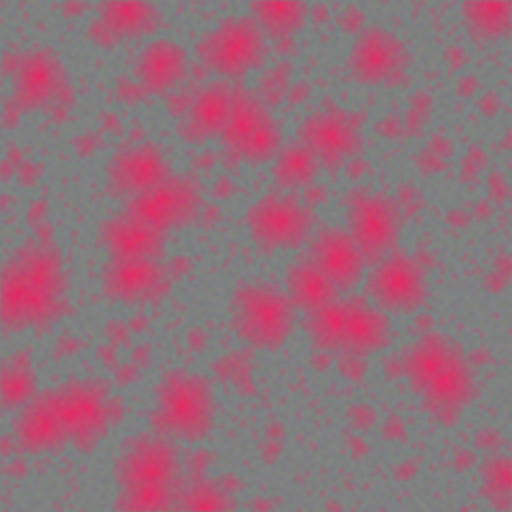
\includegraphics[width = 2in]{resources/vgg_mean_res/block1_conv1_5.png}} 
~
\subfloat[Wizualizacja filtra nr 15 bloku 1]{
\includegraphics[width = 2in]{resources/vgg_mean_res/block1_conv1_15.png}} 
~
\subfloat[Wizualizacja filtra nr 9 bloku 1]{
\includegraphics[width = 2in]{resources/vgg_mean_res/block1_conv1_9.png}} 
\\
\subfloat[Wizualizacja filtra nr 50 bloku 2]{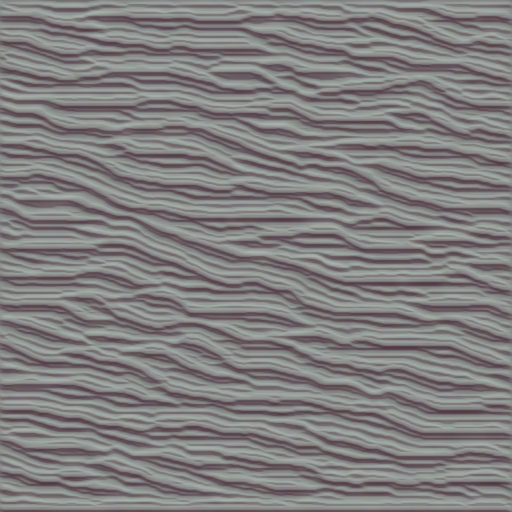
\includegraphics[width = 2in]{resources/vgg_mean_res/block1_conv2_50.png}} 
~
\subfloat[Wizualizacja filtra nr 32 bloku 2]{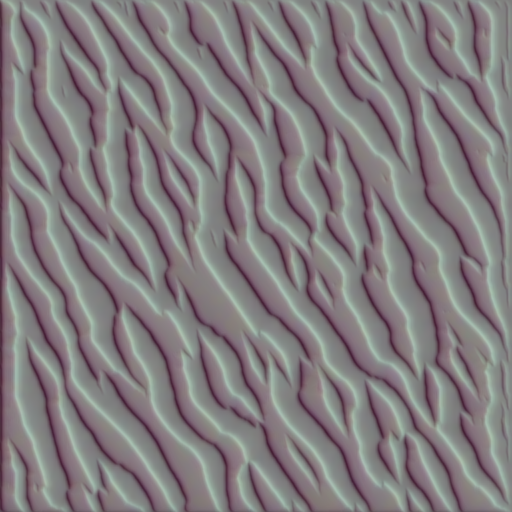
\includegraphics[width = 2in]{resources/vgg_mean_res/block1_conv2_32.png}} 
~
\subfloat[Wizualizacja filtra nr 33 bloku 2]{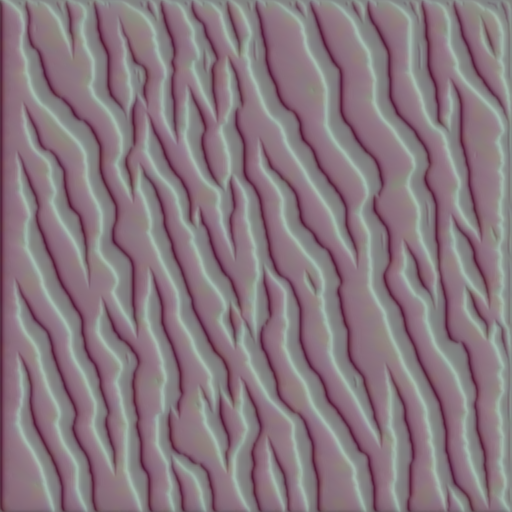
\includegraphics[width = 2in]{resources/vgg_mean_res/block1_conv2_33.png}} 
\\
\subfloat[Wizualizacja filtra nr 59 bloku 2]{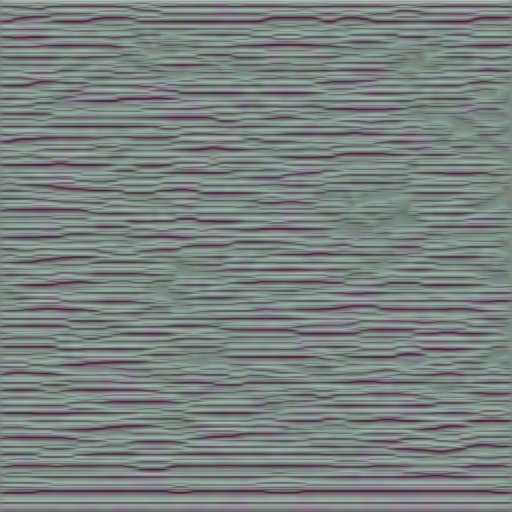
\includegraphics[width = 2in]{resources/vgg_mean_res/block1_conv2_59.png}} 
~
\subfloat[Wizualizacja filtra nr 60 bloku 2]{
\includegraphics[width = 2in]{resources/vgg_mean_res/block1_conv2_60.png}} 
~
\subfloat[Wizualizacja filtra nr 61 bloku 2]{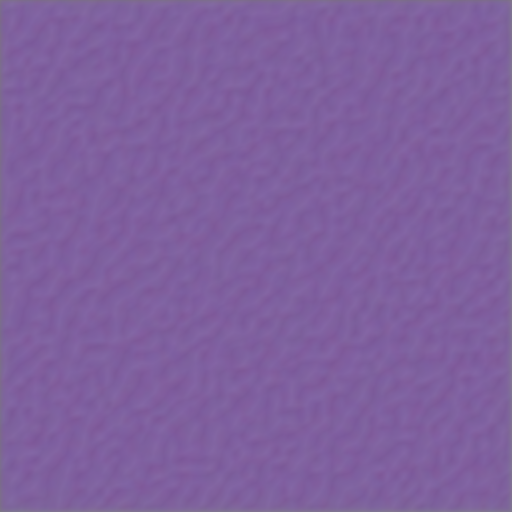
\includegraphics[width = 2in]{resources/vgg_mean_res/block1_conv2_61.png}} 
\caption{Wybrane wizualizacje warstwy sieci VGG-19 oznaczonej na rysunku \ref{vgg-model} jako conv1}
\label{mean-vgg-vis-c1bx}
\end{figure}

\begin{figure}
\subfloat[Wizualizacja filtra nr 120 bloku 2]{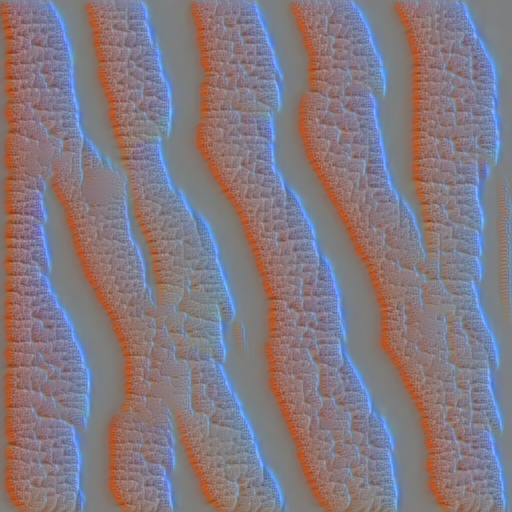
\includegraphics[width = 2in]{resources/vgg_mean_res/block2_conv2_120.png}} 
~
\subfloat[Wizualizacja filtra nr 60 bloku 2]{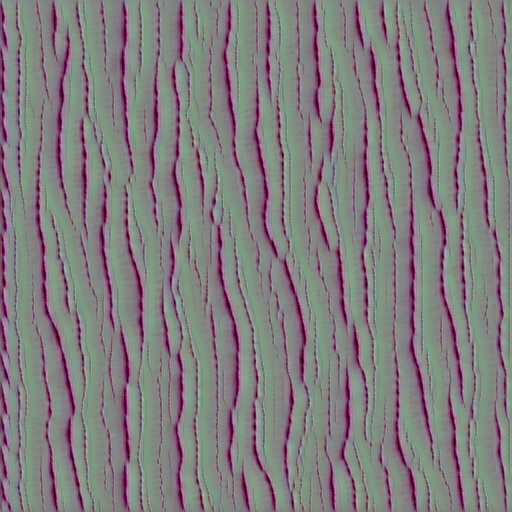
\includegraphics[width = 2in]{resources/vgg_mean_res/block2_conv2_60.png}} 
~
\subfloat[Wizualizacja filtra nr 80 bloku 2]{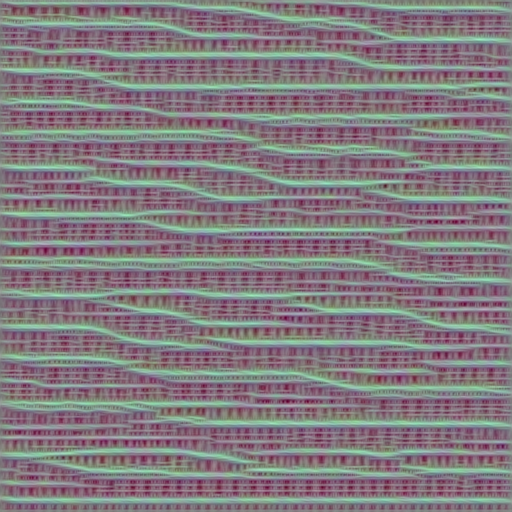
\includegraphics[width = 2in]{resources/vgg_mean_res/block2_conv2_80.png}} 
\\
\subfloat[Wizualizacja filtra nr 33 bloku 1]{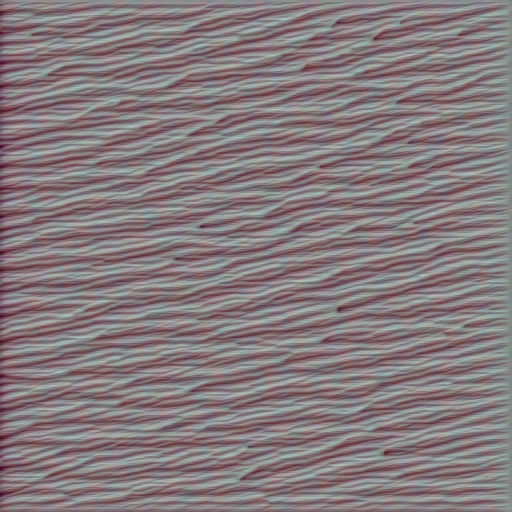
\includegraphics[width = 2in]{resources/vgg_mean_res/block2_conv1_33.png}} 
~
\subfloat[Wizualizacja filtra nr 32 bloku 1]{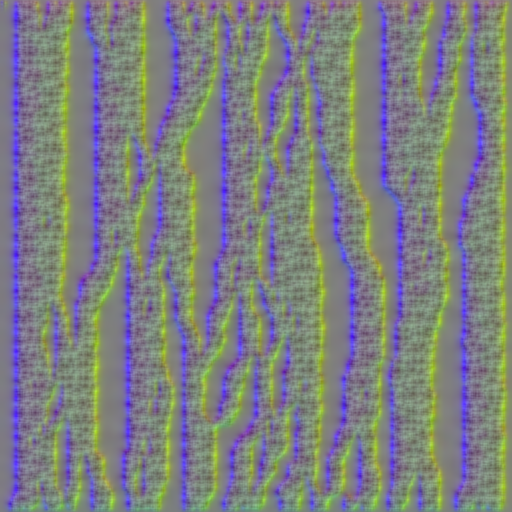
\includegraphics[width = 2in]{resources/vgg_mean_res/block2_conv1_32.png}} 
~
\subfloat[Wizualizacja filtra nr 19 bloku 1]{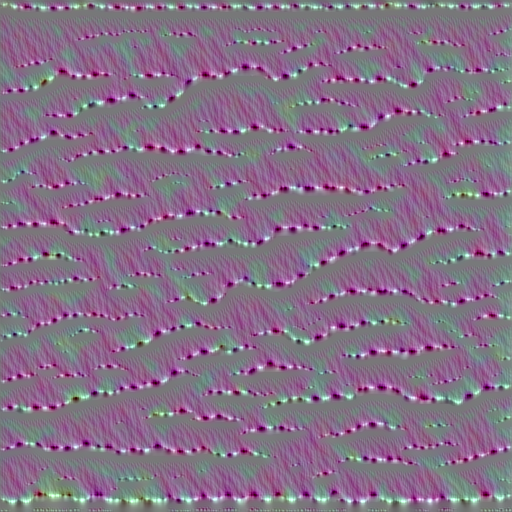
\includegraphics[width = 2in]{resources/vgg_mean_res/block2_conv1_19.png}} 
\\
\subfloat[Wizualizacja filtra nr 63 bloku 2]{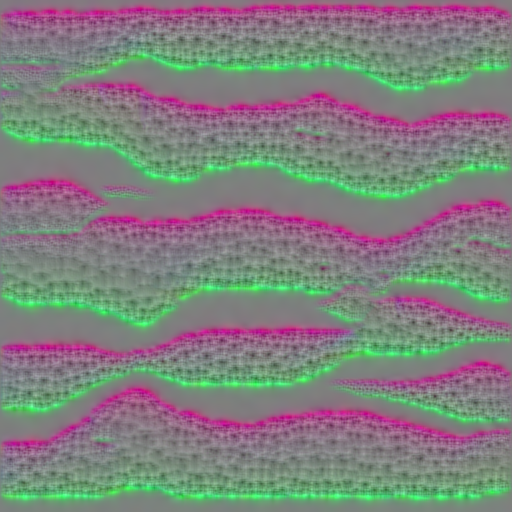
\includegraphics[width = 2in]{resources/vgg_mean_res/block2_conv2_63.png}} 
~
\subfloat[Wizualizacja filtra nr 64 bloku 2]{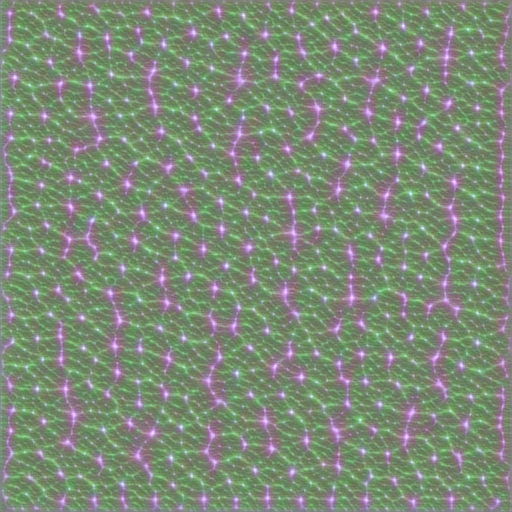
\includegraphics[width = 2in]{resources/vgg_mean_res/block2_conv2_64.png}} 
~
\subfloat[Wizualizacja filtra nr 65 bloku 2]{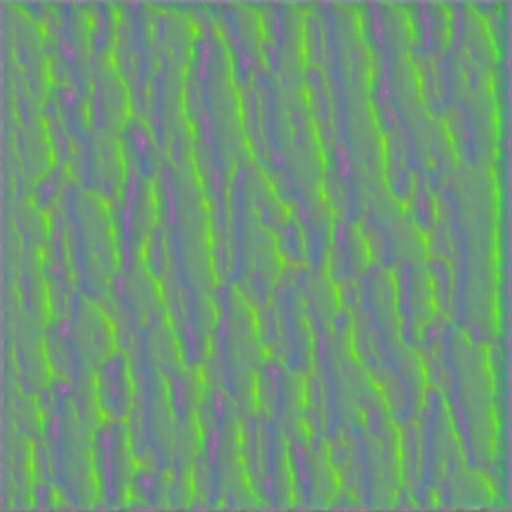
\includegraphics[width = 2in]{resources/vgg_mean_res/block2_conv2_65.png}} 

\caption{Wybrane wizualizacje warstwy sieci VGG-19 oznaczonej na rysunku \ref{vgg-model} jako conv2}
\label{mean-vgg-vis-c2bx}
\end{figure}

\begin{figure}
\subfloat[Wizualizacja filtra nr 128 bloku 4]{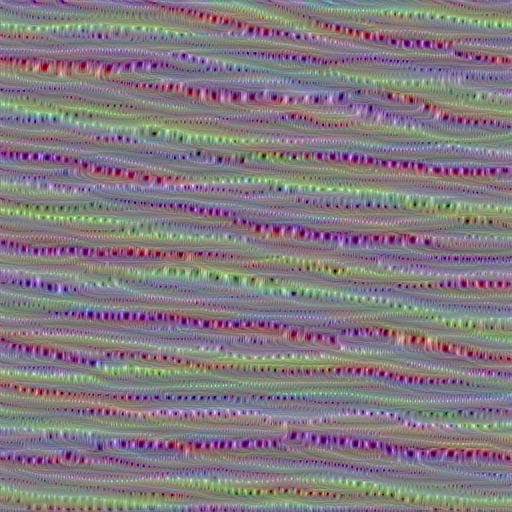
\includegraphics[width = 2in]{resources/vgg_mean_res/block3_conv4_128.png}} 
~
\subfloat[Wizualizacja filtra nr 17 bloku 4]{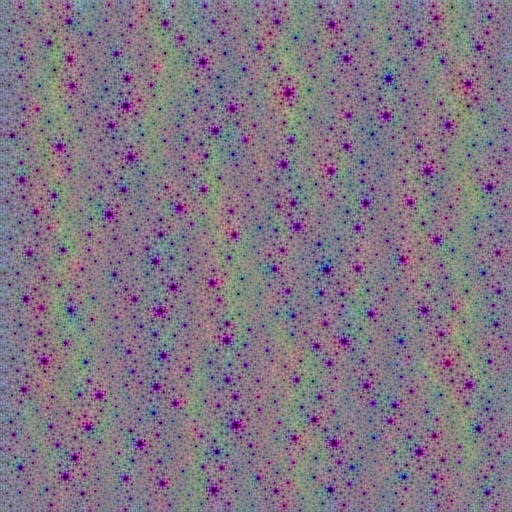
\includegraphics[width = 2in]{resources/vgg_mean_res/block3_conv4_17.png}} 
~
\subfloat[Wizualizacja filtra nr 9 bloku 2]{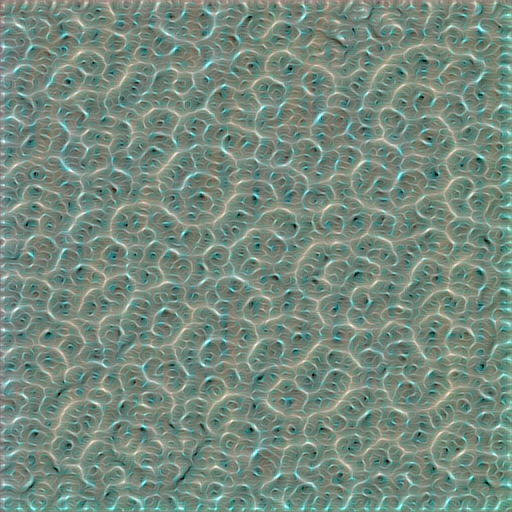
\includegraphics[width = 2in]{resources/vgg_mean_res/block3_conv2_9.png}} 
\\
\subfloat[Wizualizacja filtra nr 34 bloku 3]{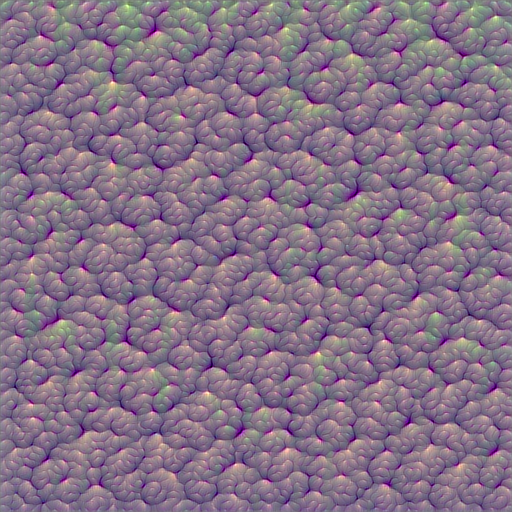
\includegraphics[width = 2in]{resources/vgg_mean_res/block3_conv3_34.png}} 
~
\subfloat[Wizualizacja filtra nr 15 bloku 1]{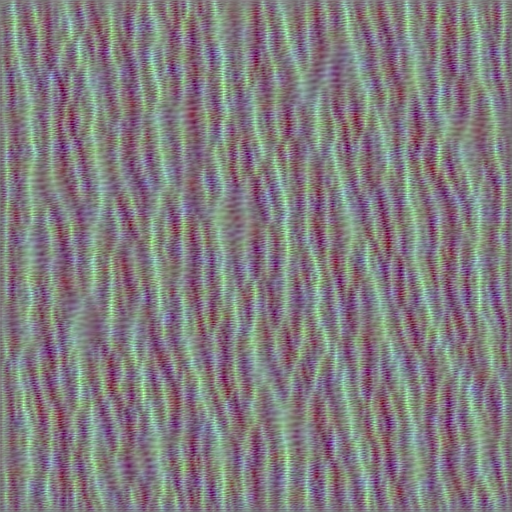
\includegraphics[width = 2in]{resources/vgg_mean_res/block3_conv1_15.png}} 
~
\subfloat[Wizualizacja filtra nr 32 bloku 3]{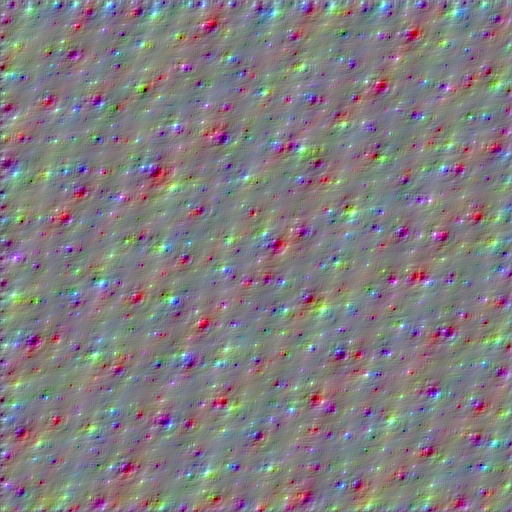
\includegraphics[width = 2in]{resources/vgg_mean_res/block3_conv3_32.png}} 
\\
\subfloat[Wizualizacja filtra nr 254 bloku 4]{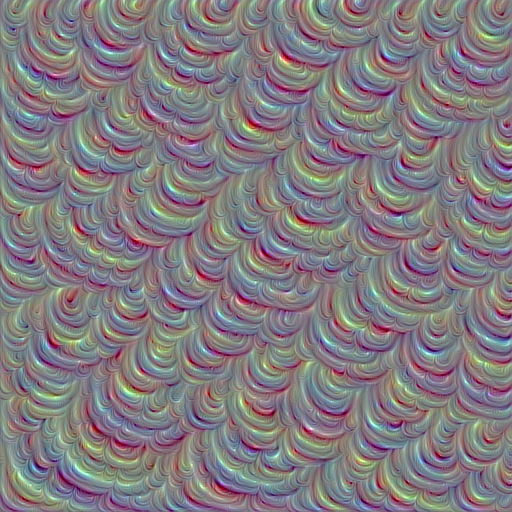
\includegraphics[width = 2in]{resources/vgg_mean_res/block3_conv4_254.png}} 
~
\subfloat[Wizualizacja filtra nr 32 bloku 4]{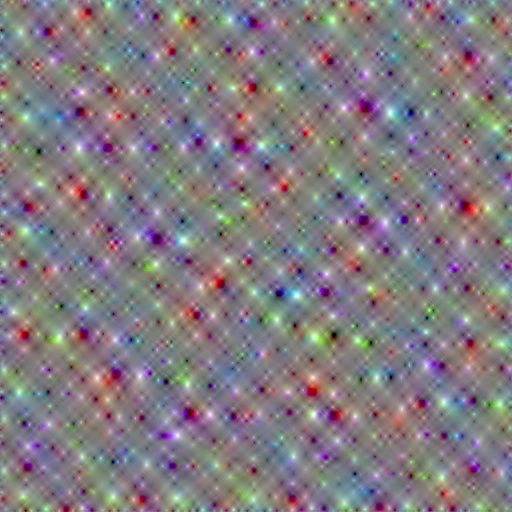
\includegraphics[width = 2in]{resources/vgg_mean_res/block3_conv4_32.png}} 
~
\subfloat[Wizualizacja filtra nr 33 bloku 4]{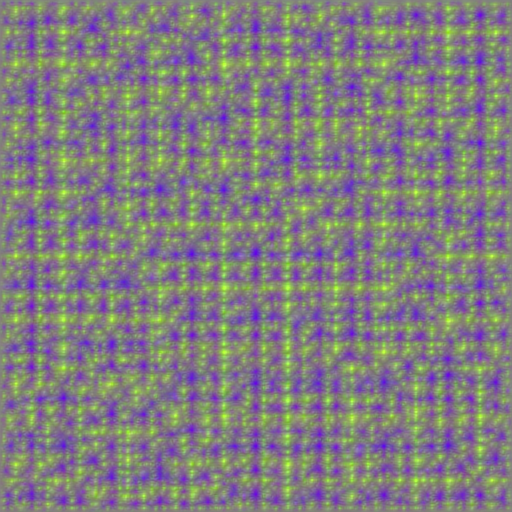
\includegraphics[width = 2in]{resources/vgg_mean_res/block3_conv1_59.png}} 

\caption{Wybrane wizualizacje warstwy sieci VGG-19 oznaczonej na rysunku \ref{vgg-model} jako conv3}
\label{mean-vgg-vis-c3bx}
\end{figure}

\begin{figure}
\subfloat[Wizualizacja filtra nr 128 bloku 4]{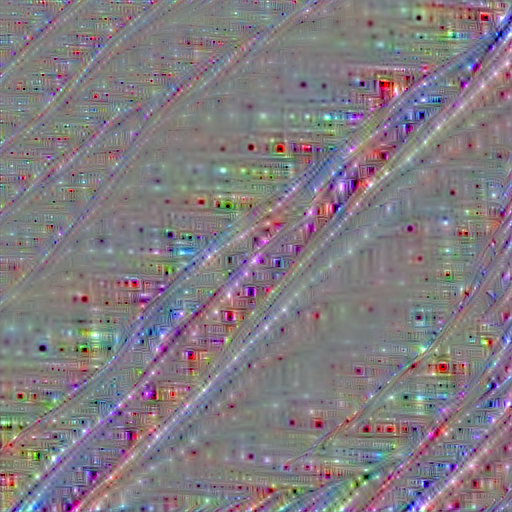
\includegraphics[width = 2in]{resources/vgg_mean_res/block4_conv4_128.png}} 
~
\subfloat[Wizualizacja filtra nr 17 bloku 4]{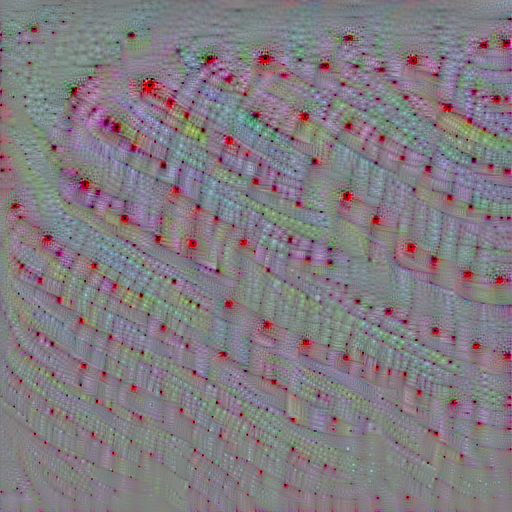
\includegraphics[width = 2in]{resources/vgg_mean_res/block4_conv4_17.png}} 
~
\subfloat[Wizualizacja filtra nr 32 bloku 4]{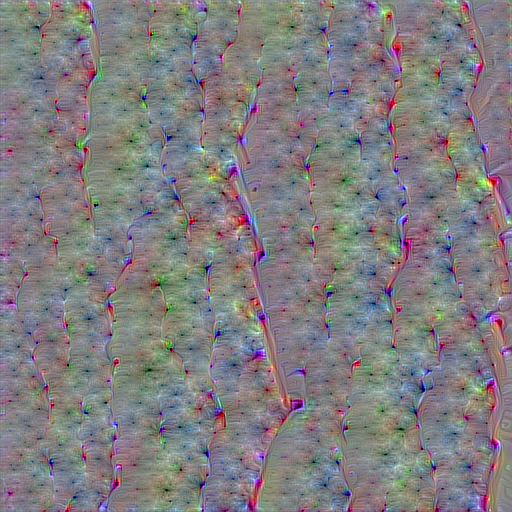
\includegraphics[width = 2in]{resources/vgg_mean_res/block4_conv4_32.png}} 
\\
\subfloat[Wizualizacja filtra nr 10 bloku 1]{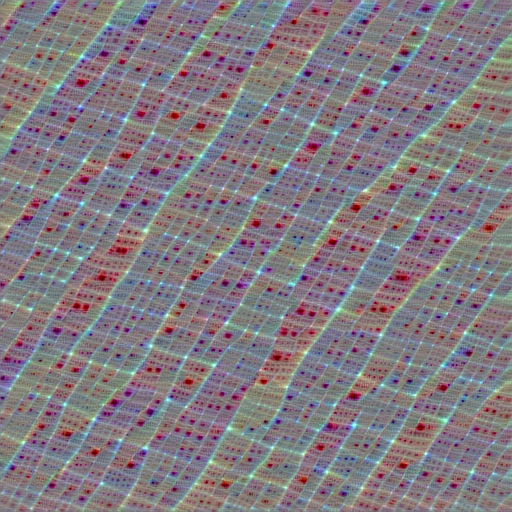
\includegraphics[width = 2in]{resources/vgg_mean_res/block4_conv1_10.png}} 
~
\subfloat[Wizualizacja filtra nr 11 bloku 2]{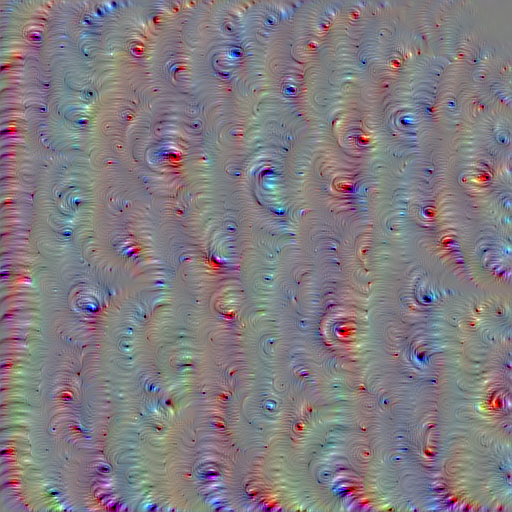
\includegraphics[width = 2in]{resources/vgg_mean_res/block4_conv2_11.png}} 
~
\subfloat[Wizualizacja filtra nr 15 bloku 3]{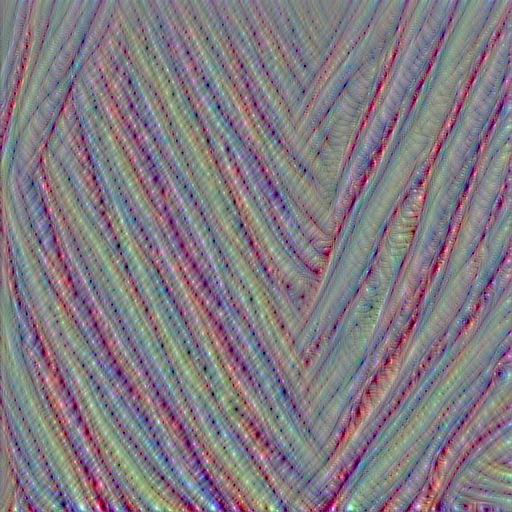
\includegraphics[width = 2in]{resources/vgg_mean_res/block4_conv3_15.png}} 
\\
\subfloat[Wizualizacja filtra nr 59 bloku 1]{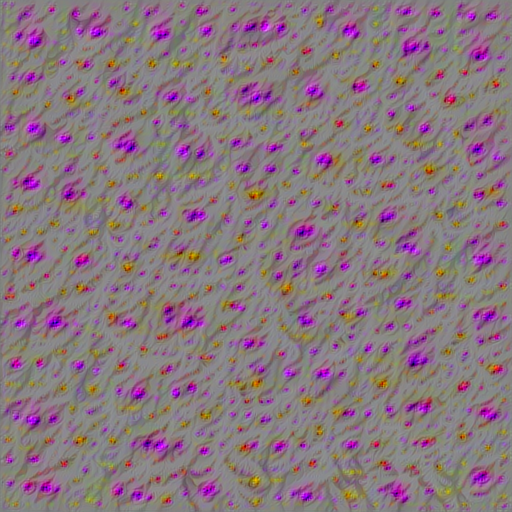
\includegraphics[width = 2in]{resources/vgg_mean_res/block4_conv1_59.png}} 
~
\subfloat[Wizualizacja filtra nr 64 bloku 2]{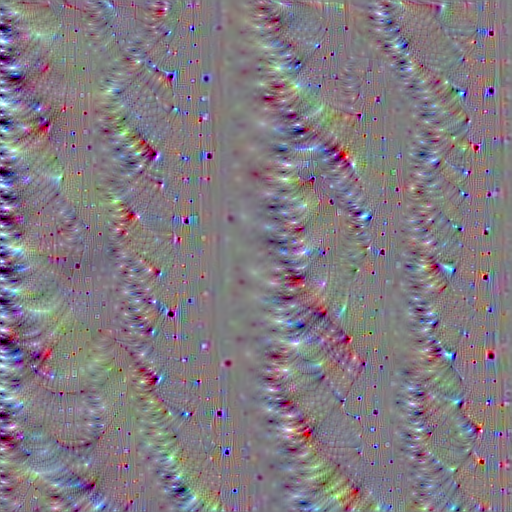
\includegraphics[width = 2in]{resources/vgg_mean_res/block4_conv2_64.png}} 
~
\subfloat[Wizualizacja filtra nr 65 bloku 3]{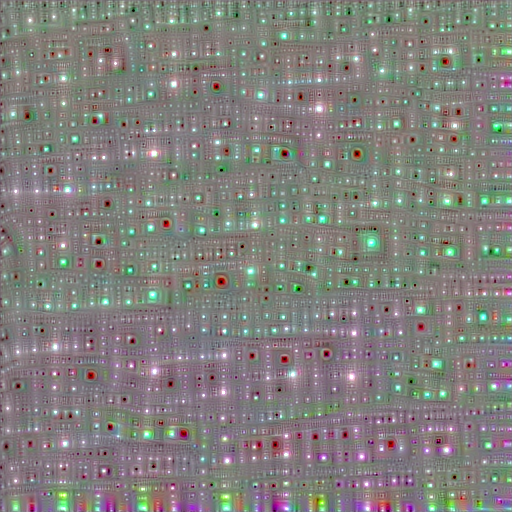
\includegraphics[width = 2in]{resources/vgg_mean_res/block4_conv3_65.png}} 

\caption{Wybrane wizualizacje początkowej warstwy sieci VGG-19 (oznaczonej na rysunku \ref{vgg-model} jako conv4)}
\label{mean-vgg-vis-c4bx}
\end{figure}

\begin{figure}
\subfloat[Wizualizacja filtra nr 120 bloku 1]{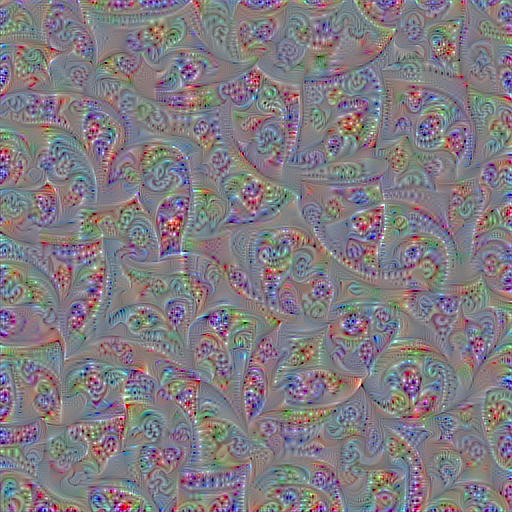
\includegraphics[width = 2in]{resources/vgg_mean_res/block5_conv1_120.png}} 
~
\subfloat[Wizualizacja filtra nr 3 bloku 1]{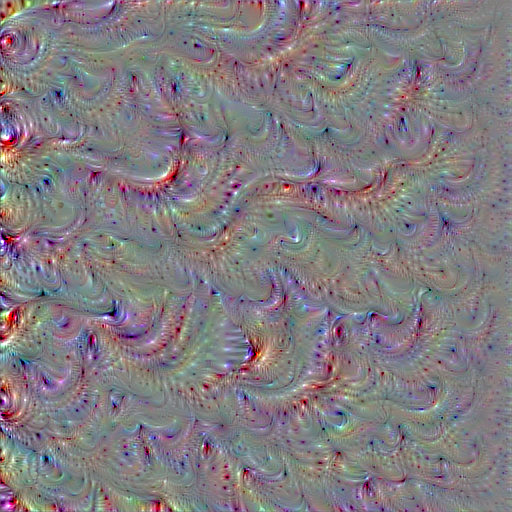
\includegraphics[width = 2in]{resources/vgg_mean_res/block5_conv1_3.png}} 
~
\subfloat[Wizualizacja filtra nr 30 bloku 1]{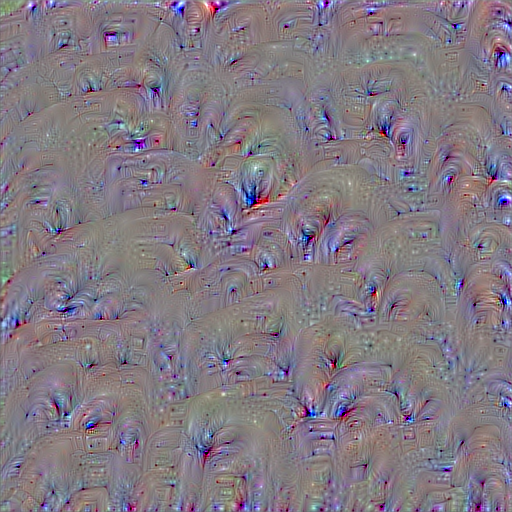
\includegraphics[width = 2in]{resources/vgg_mean_res/block5_conv1_30.png}} 
\\
\subfloat[Wizualizacja filtra nr 60 bloku 1]{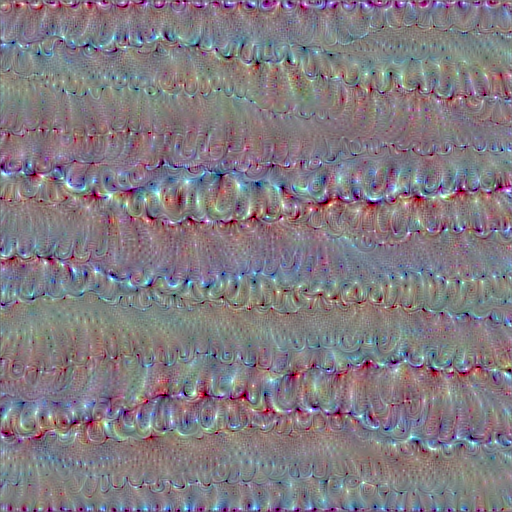
\includegraphics[width = 2in]{resources/vgg_mean_res/block5_conv1_60.png}} 
~
\subfloat[Wizualizacja filtra nr 60 bloku 2]{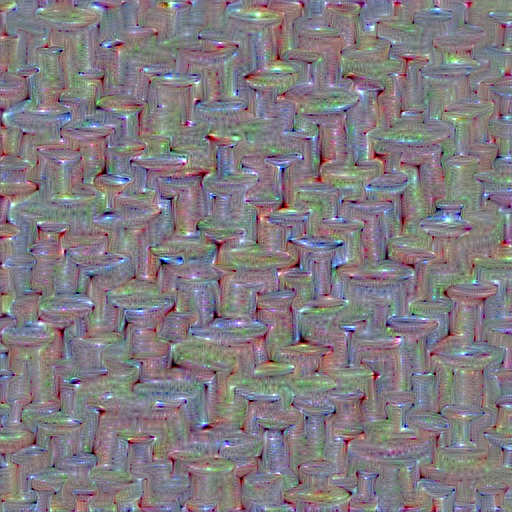
\includegraphics[width = 2in]{resources/vgg_mean_res/block5_conv2_60.png}} 
~
\subfloat[Wizualizacja filtra nr 63 bloku 4]{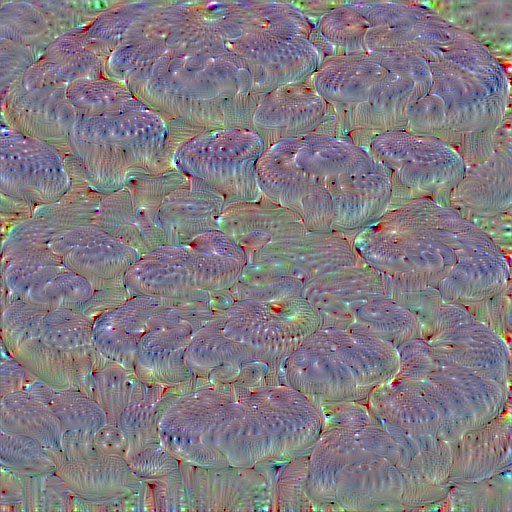
\includegraphics[width = 2in]{resources/vgg_mean_res/block5_conv4_63.png}} 
\\
\subfloat[Wizualizacja filtra nr 63 bloku 2]{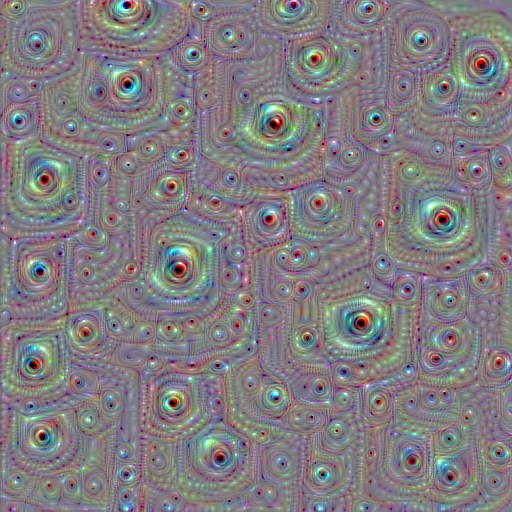
\includegraphics[width = 2in]{resources/vgg_mean_res/block5_conv2_63.png}} 
~
\subfloat[Wizualizacja filtra nr 90 bloku 1]{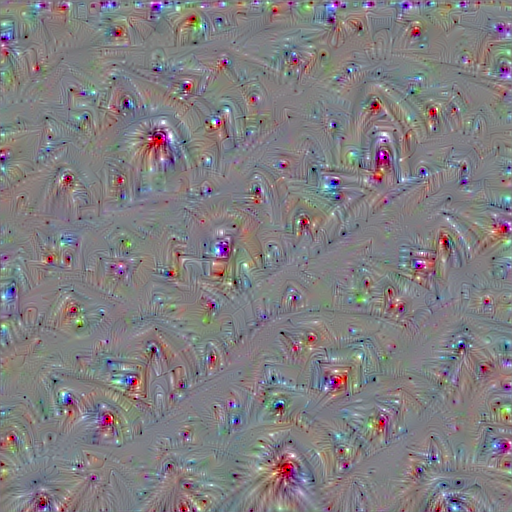
\includegraphics[width = 2in]{resources/vgg_mean_res/block5_conv1_90.png}} 
~
\subfloat[Wizualizacja filtra nr 65 bloku 4]{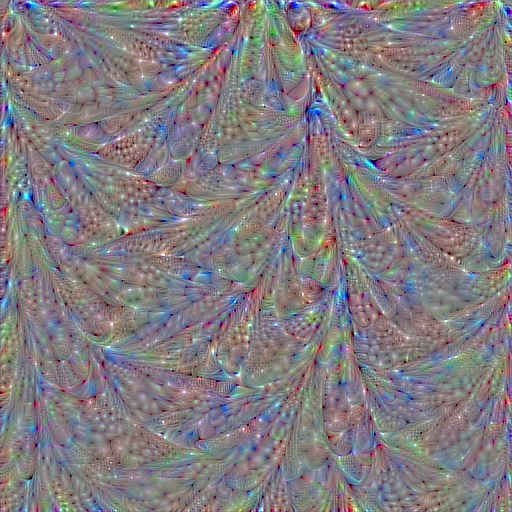
\includegraphics[width = 2in]{resources/vgg_mean_res/block5_conv4_65.png}} 
\caption{Wybrane wizualizacje warstwy sieci VGG-19 oznaczonej na rysunku \ref{vgg-model} jako conv5}
\label{mean-vgg-vis-c5bx}
\end{figure}

\subsection{Wizualizacja maksymalnej aktywacji danej klasy}
\label{vgg-class-visualisation}

VGG19 w inny od człowieka sposób uchwyca to czym jest dany na obrazie przedmiot. By zwizualizować w jaki sposób sieć odróżnia poszczególne klasy, można posłużyć się analogicznym sposóbem postępowania jak z podrozdziału \ref{vgg-mean-activation}.
Jeżeli do modelu przywrócićby warstwy gęste i próbować zmaksymalizować aktywację dla jednej z klas poprzez modyfikację obrazu wejściowego, powinienem otrzymać obraz, który sieć bezwątpliwie traktowałaby jako reprezentanta danej klasy.
Gdyby sieć miała w sobie zakodowaną informację o tym co tak naprawdę jest na obrazie powinienem otrzymać coś przynajmniej odlegle przypominającego oryginalną klasę.

Weźmy przykładowo klasę numer 319 w przypadku tego konkretnego modelu odpowiada ona klasie ważki. 

\begin{figure}[ht]
\centerline{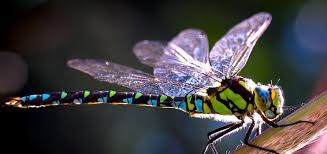
\includegraphics[scale=0.8]{resources/vgg_mean_topincluded/dragonfly.jpeg}}
\caption{Przykładowe zdjęcie ważki.}
\label{fig:wazka-real}
\end{figure}

\label{lst:wazka-prediction}
\begin{lstlisting}[language=Python, caption={Predykcja klasy zdjęcia ważki\ref{fig:wazka-real}.}, captionpos=b]
img = image.load_img('resources/vgg_mean_topincluded/dragonfly.jpeg', target_size=(224, 224))
x = image.img_to_array(img)
x = np.expand_dims(x, axis=0)
x = preprocess_input(x)
preds = model.predict(x)
print('Predicted:', decode_predictions(preds, top=3)[0])
\end{lstlisting}

\label{lst:wazka-prediction-result}
\begin{lstlisting}[language=Python, caption={Wynik skryptu \ref{lst:wazka-prediction}.}, captionpos=b]
[('n02268443', 'dragonfly', 0.96805733), ('n02268853', 'damselfly', 0.01810956), ('n02264363', 'lacewing', 0.012446008)]
\end{lstlisting}

Oznacza to nie mniej, że sieć którą dysponuję jest przekonana, w zaokrągleniu, na 97\% mamy do czynienia z ważką. Dwie kolejne najbardziej prawdopodobne klasy przedstawiają inny rodzaj ważki - ważkę równoskrzydłą i owada siatkoskrzydłego.

Wszystko wydaje się być w porządku dopóki nie wygenerujemy obrazu na podstawie wyżej wymienionej klasy. Uprzednio modyfikując funkcję kosztu, tak by teraz zwracała wartość jaką przypisuje klasie ważki softmax, możemy zmodyfikować szary szum tak by maksymalizować (wg. sieci) prawdopodobieństwo tego, że na obrazie jest ważka. Tym nie skaluje obrazu podczas treningu i modyfikuję obraz \(224 \times 224\).

\begin{figure}[ht]
\centerline{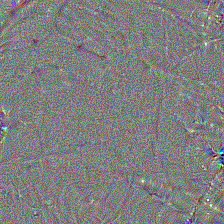
\includegraphics[scale=0.8]{resources/vgg_mean_topincluded/dragonfly-fake.png}}
\caption{Ważka uzyskana w odwróconym procesie treningu.}
\label{fig:wazka-fake}
\end{figure}

Mimo krótkiego czasu treningu taki obraz klasyfikowany jest przez sieć VGG19 jako ważka z pewnością sięgającą 96\%. Podobny wynik uzyskałem na wszystkich testowanych przeze mnie klasach. VGG rozpoznaje przedmioty na podstawie prawdopodobieństwa wystąpienia pewnej kombinacji filtrów - niestety samo nie nadaje się do generowania realistycznych obrazów danej klasy. 
By uzyskać obrazy zdolne do oszukania ludzkiej percepcji należy posłużyć się architekturą typu GAN (\textit{ang. Generative Adversarial Networks}).

Niezwykle zajmującym tematem wydaje się być próba wprowadzenia uzyskanych wizualizacji do sieci VGG i uzyskanie odpowiedzi samej sieci co jest na danym obrazie. 
Zmuszony jednak jestem zostawić temat wizualizacji uzyskanych za pomocą maksymalizacji aktywacji warstwy na rzecz innego zajmującego tematu - neuronowego transferu stylu.

\section{\textit{Neural Style Transfer} przy pomocy sieci VGG}
\label{vgg-nst}
\textit{Neural Style Transfer} został pierwszy raz zaprezentowany w pracy autorstwa Leon A. Gatys, Alexander S. Ecker, Matthias Bethge \cite{nstpaper}.
Jest to technika mająca na celu uzyskanie obrazu \(G\) w stylu obrazu \(S\), przy pomocy obrazu bazowego \(B\) \ref{neural-style-transfer-BSG}.

Jej oryginalni autorzy sami podają kluczową obserwację, umożliwiającą mieszanie obrazu. Jest to spostrzeżenie, że możliwe jest odesparowanie stylu
i treści z zakodowanej w aktywacjach sieci VGG.

Załóżmy, że chcemy za pomocą wybranej warstwy konwolucyjnej sieci VGG odzwierciedlić treść obrazu \(C\) na obrazie \(G\). Mamy do wyboru warstwy oznaczone conv1...5.
Gdy wybierzemy jedną warstwę i wykonamy dla obrazów \(C\) i \(G\) kroki propagacji w przód otrzymamy mapy aktywacji \(a_{C}\) i \(a_{G}\). Korzystając z nich, można zdefiniować
funkcję kosztu: \[J_{c}^{[l]}(C, G) = \frac{1}{4 \times n_H \times n_W \times n_F} \sum{(a_{C} - a_{G})^{2}} \]

Gdzie:

\begin{itemize}
\item
    \(n_{W}\) -- szerokość filtra wybranej warstwy,
\item
    \(n_{H}\) -- wysokość filtra wybranej warstwy,
\item
    \(n_{F}\) -- ilość filtrów wybranej warstwy,
\item
    \(l\) -- numer zastosowanej warstwy,
\end{itemize}

A sumowanie odbywa się po wszystkich elementach mapy cech (uzyskana suma jest sumą aktywacji wszystkich warstw). 

Analogicznie można potraktować problem odzwierciedlenia stylu obrazu. Po wyborze warstwy uzyskujemy aktywację dla obrazów \(S\) i \(G\) oraz oznaczamy je kolejno \(a_{S}\) i \(a_{G}\). 
Następnie zwijamy tensory o wymiarach \(n_H \times n_W \times n_F\) w dwuwymiarowe macierze o wymiarach \((n_H + n_W) \times n_F\) i wyznaczamy macierze Grama tych macierzy, oznaczamy je jako 
\(G^{(S)}\) i \(G^{(G)}\). Wtedy można zdefiniować następującą funkcję kosztu stylu.

\[J_{s}^{[l]}(S,G) = \frac{1}{4 \times {n_F}^2 \times (n_H \times n_W)^2} \sum _{i=1}^{n_F}\sum_{j=1}^{n_F}(G^{(S)}_{ij} - G^{(G)}_{ij})^2\tag{2}\]

Gdy zdefiniujemy zbiorczą funkcję kosztu jako:

\[J(G) = \alpha J_{c}(C,G) + \beta J_{s}(S,G)\]

Gdzie:
\begin{itemize}
\item
    \(\alpha\) -- współczynnik kosztu treści,
\item
    \(\beta\) -- współczynnik kosztu stylu,
\end{itemize}

Sterując \(\alpha\) i \(\beta\) można wpływać na to jak bardzo obraz będzie wierny orginałowi \textit{C} w stosunku do jak bardzo będzie namalowany w stylu \textit{S}. Używając tak zdefiniowanej funkcji kosztu dla jednej 
z warstw, można zapisać funkcję biorącą pod uwagę wyjście z kilku warstw konwolucyjnych jednocześnie: 

\[J_{s}(S,G) = \sum_{l} \lambda^{[l]} J^{[l]}_{s}(S,G) \]

Gdzie \(\lambda^{[l]}\) jest współczynnikiem wykorzystania danej warstwy \(l\).

Przy pomocy tej funkcji, można zastosować sposób działania znany z podrozdziału \ref{vgg-mean-activation}. Używając ją zamiast mediany aktywacji danej warstwy uzyskamy efekt widoczny na rysunku \ref{neural-style-transfer-BSG}. Szczegół implementacyjny: zaprezentowany obraz został wygenerowany przy pomocy skryptu napisanego w \textit{tensorflow} a nie na podstawie modyfikacji opisanego wyżej skryptu.
Powód jest ściśle praktyczny, dysponowałem już takim skryptem mojego autorstwa - nie było praktyczne jednak wprowadzanie nowej biblioteki uczenia maszynowego, a jak było napisane wyżej, identyczne efekty można uzyskać przy pomocy Kerasa.

\begin{figure}
\subfloat[Obraz bazowy (B), autor zdjęcia: Grzegorz Rucki]{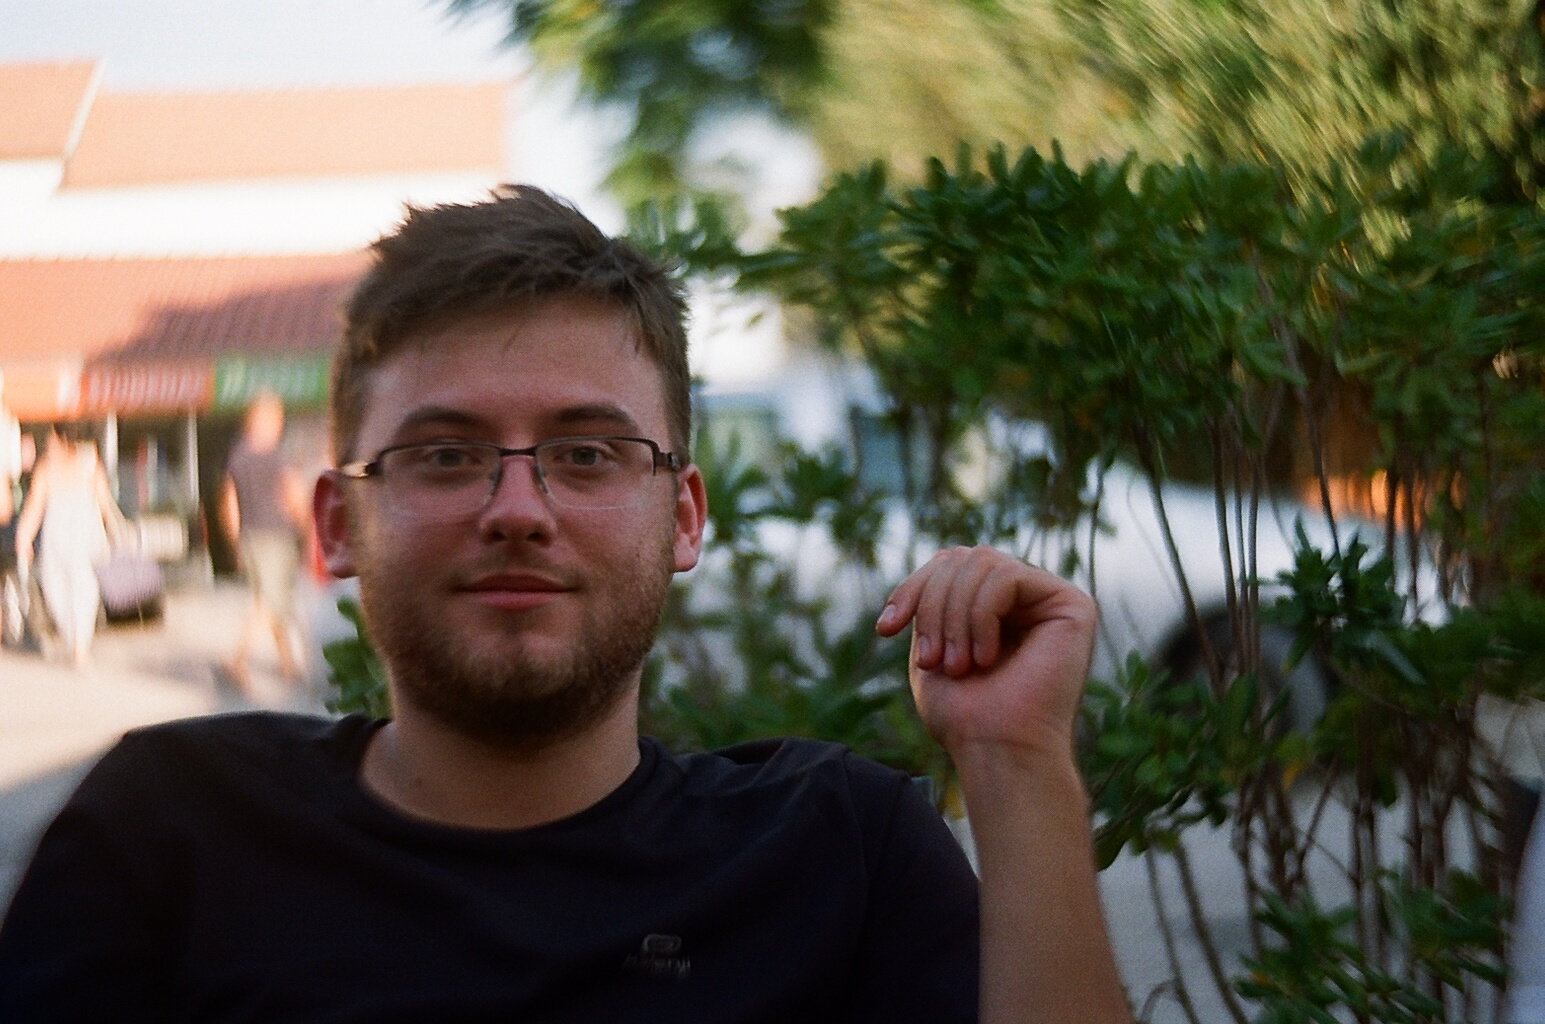
\includegraphics[width = 3in]{resources/nst/69850020.JPG}} 
~
\subfloat[Obraz stylu (S), ekpresjonistyczny - ''The keep''\cite{thekeep}]{\includegraphics[width = 2in]{resources/nst/the_keep_1958.jpg}} 
\\
\subfloat[Wygenerowany obraz (G)]{\includegraphics[width = 5in]{resources/nst/nst__at_iteration_9.png}} 
\caption{Transfer stylu na przykładzie zdjęcia z wakacji.}
\label{neural-style-transfer-BSG}
\end{figure}

